\section{Vorstellung}
\label{sec:VorstellungBD4B}  

In this section we describe the \ac{JBI} \ac{BC}s shipped in the ServiceMix-mt prototype this diploma thesis focuses on, and the transport protocols they support. 



ServiceMix provides \ac{HTTP} communication support in its \ac{HTTP} \ac{JBI} \ac{BC}. Its \ac{HTTP} consumer and provider endpoints are built on the \ac{HTTP} Jetty 6 server and Jakarta Commons \ac{HTTP} Client respectively, providing support for both REST and SOAP over HTTP 1.1 and 1.2 requests.

The original \ac{HTTP} \ac{BC} is extended in the ServiceMix-mt prototype to provide multi-tenant support in \cite{Muhler2012} and \cite{gomez2012}. Muhler provides an internal dynamic creation of tenant-aware endpoints in the \ac{BC}, by injecting tenant context in the \ac{JBI} endpoint's URLs \cite{Muhler2012}. Gomez provides a \ac{NMF} with tenant context information in its properties for routing in the \ac{NMR} \cite{gomez2012}. However, in this diploma thesis we must not only provide tenant isolation at the tenant level, but also isolation at the user level. We discuss this requirement in detail in Chapters \ref{chap:spec} and \ref{chap:design}.

\begin{figure}[htb]
	\centering
		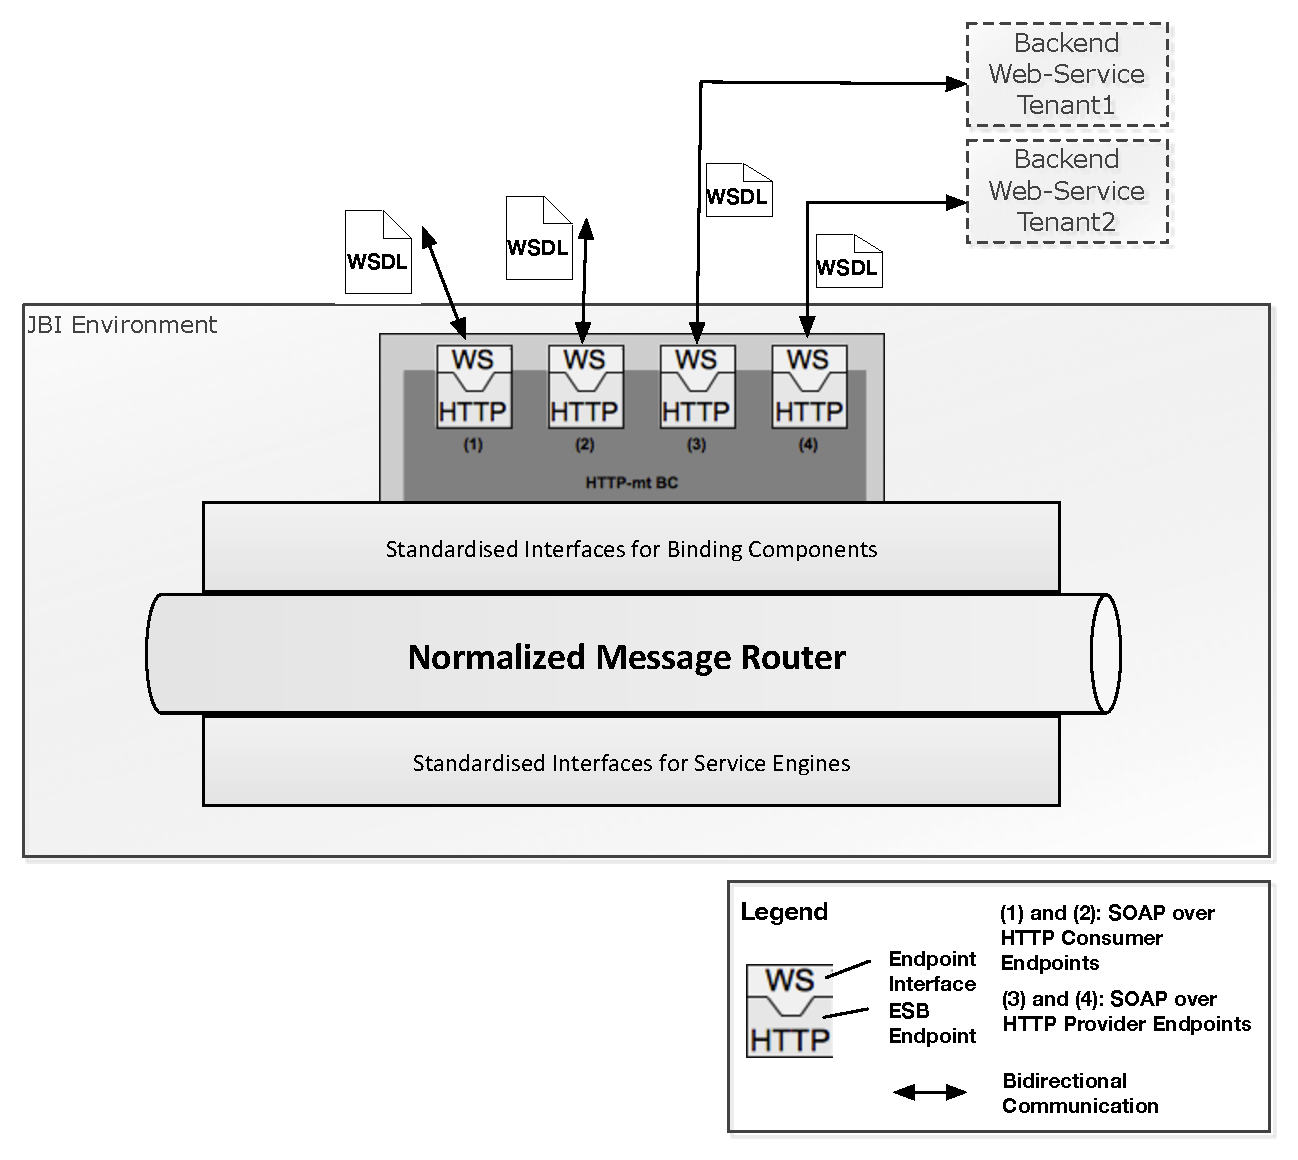
\includegraphics[clip, scale=0.3]{./gfx/httpmtbc.pdf}
	\caption[Multi-tenant HTTP Binding Component]{Multi-tenant HTTP Binding Component \cite{gomez2012}. }
	\label{fig:httpmt}
\end{figure}

As seen in Figure \ref{fig:httpmt}, the multi-tenant \ac{HTTP} \ac{BC} is mainly used in ServiceMix-mt to support the \ac{SOAP} over \ac{HTTP} communication protocol by exposing a Web service in the tenant-aware consumer endpoint and consuming an external Web service in the provider endpoint. \ac{SOAP} defines an \ac{XML} message format  which is sent over the network and a set of rules for processing the \ac{SOAP} message in the different \ac{SOAP} nodes which build the message path between two endpoints \cite{Weera2005}. A \ac{SOAP} message is a composition of three main elements: a SOAP envelope, header, and body. A SOAP envelope may contain zero or more headers and one body. The header may contain processing or authentication data for the ultimate receiver or for the intermediate nodes through the message is routed. The message payload or business data is included in the SOAP body. SOAP is used as a message framework for accessing Web services in loosely coupled infrastructures \cite{Weera2005}. The Web service consumer specifies the functionality to invoke in the SOAP body. If the Web service functionality has a request-response \ac{MEP}, a SOAP message is used to send the response data when the corresponding operation has been executed successfully or the error data in case an error occurred during execution.

Most of the Cloud storage providers provide an \ac{HTTP} interface to the tenants for data management, retrieval, and storage. In this diploma thesis we extend this \ac{JBI} \ac{BC} in order to provide the tenant a transparent access to his \ac{NoSQL} Cloud data stores.

\FloatBarrier
